\chapter{Advanced simulations}\label{advance}

\vk
In this chapter, advice to perform more sophisticated simulations is provided to advanced users. 

\mk
\section{Running nested simulations}\label{nests}

\paragraph{Preparing namelist.input} For simulations with \ttt{max\_dom} nested domains, \ttt{max\_dom} parameters must be set wherever there is a ``," in the \ttt{namelist.input\_full} template in chapter~\ref{zeparam}. Specific parameters for nested simulations are labelled with \ttt{(n)} in this \ttt{namelist.input} template (see e.g. categories \ttt{\&time\_control}, \ttt{\&domains} and \ttt{\&bdy\_control}). To help you with filling the \ttt{namelist.input} file for a nested simulation, a commented example is given below. 

\vskip -0.4cm
\scriptsize
\codesource{namelist.input_nests}
\normalsize

\paragraph{Preparing namelist.wps} As is the case for single-domain simulations, the common parameters in the two files \ttt{namelist.input} and~\ttt{namelist.wps} must be exactly similar. Similarly to single-domain simulations, an automated generation of \ttt{namelist.wps} from \ttt{namelist.input} is provided in the \ttt{runmeso} script. If you do not use \ttt{runmeso} to generate the \ttt{namelist.wps} file, please bear in mind that in this file, dates are different for the parent domain and the child domains, since boundary conditions are needed only for the parent domain while initial conditions are needed for all domains. The \ttt{namelist.wps} file associated to the previously described \ttt{namelist.input} file is given below\footnote{You may find \ttt{namelist.input\_nests} and \ttt{namelist.wps\_nests} in \ttt{\$MMM/SIMU}.} and corresponds to a nested simulation in the Hellas Planitia region (Figure~\ref{nesteddomains}). Note that map projection is similar in all nests.

\vskip -0.2cm
\scriptsize
\codesource{namelist.wps_nests}
\normalsize

\begin{center} 
\begin{figure}[h!]
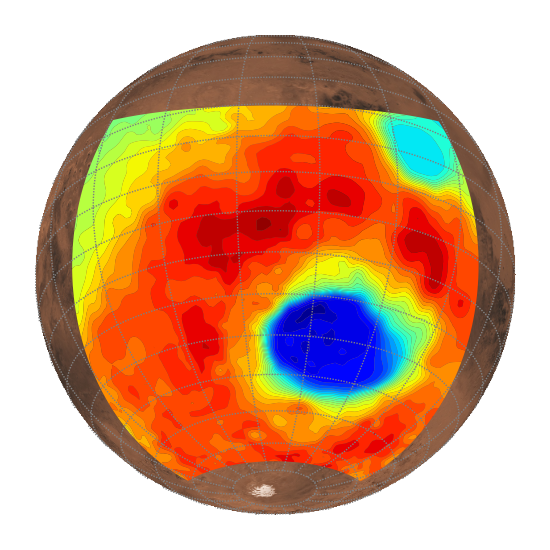
\includegraphics[width=0.33\textwidth]{LMD_MMM_d1_63km_domain_100.png} 
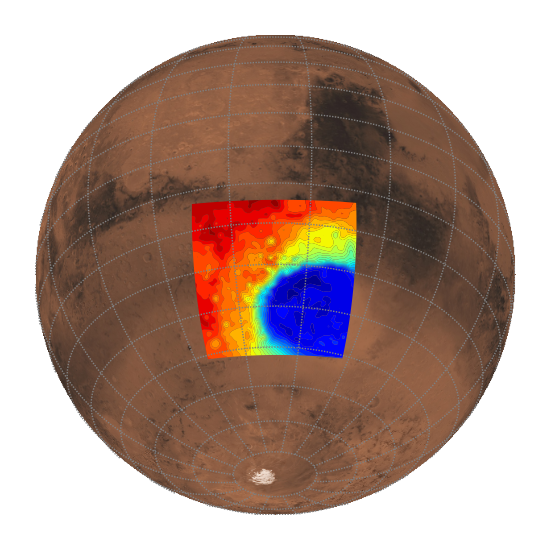
\includegraphics[width=0.33\textwidth]{LMD_MMM_d2_21km_domain_100.png}
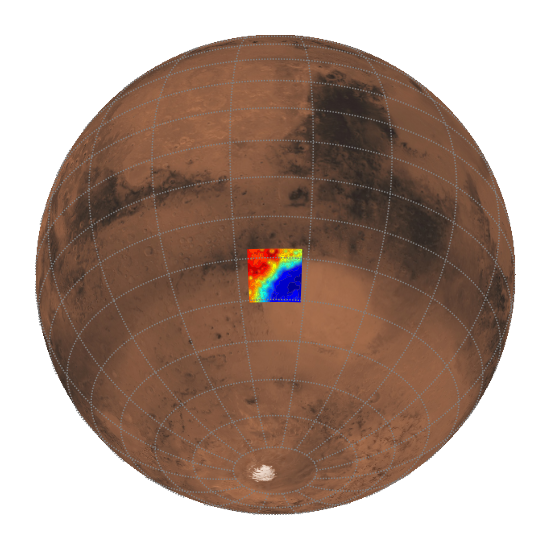
\includegraphics[width=0.33\textwidth]{LMD_MMM_d3_7km_domain_100.png}
\caption{\label{nesteddomains} Domains for a nested mesoscale simulations in Hella Planitia defined by \ttt{namelist.wps\_nests}. From left to right, ``parent" domain i.e. nest number~$1$ (horizontal resolution $63$~km), ``child" domain i.e. nest number~$2$ (horizontal resolution $21$~km), ``grandchild" domain i.e. nest number~$3$ (horizontal resolution $7$~km).}
\end{figure}
\end{center}

\paragraph{Preparing callphys.def} If you run a simulation with, say, $3$ domains, please ensure that you defined three files \ttt{callphys.def}, \ttt{callphys\_d2.def} and \ttt{callphys\_d3.def} (one per nest). If needed, different settings for physical parameterizations can be made in each nest; usually all settings in these files are similar, except \ttt{iradia} (so that differences in dynamical timesteps between nests can be potentially impacted to \ttt{callphys*.def} in order to synchronize radiative transfer call).

\paragraph{Compiling} Use the command \ttt{makemeso} and specify the number of domains and dimensions set in \ttt{namelist.input} (as far as the horizontal grid is concerned, answers to \ttt{makemeso} shall refer to the values of \ttt{e\_we} and \ttt{e\_sn} for the parent domain). This is done automatically of course if you use \ttt{runmeso} which reads the information in \ttt{namelist.input}.

\paragraph{Running} If grid nesting and parallel computing are used, no more than~$4$ processors can be used. If the nested simulation is unstable, try a single-domain simulation with the parent domain and choose best parameters for stability (e.g., \ttt{time\_step}), then add a first nested domain, and start again stability tests and investigations, etc.

\paragraph{Inputs/outputs} Defining several domains yield one output per domain: e.g. for three domains \ttt{geogrid.exe} yields \ttt{geo\_em.d01.nc}, \ttt{geo\_em.d02.nc}, \ttt{geo\_em.d03.nc}\ldots; \ttt{real.exe} yields \ttt{wrfinput\_d01}, \ttt{wrfinput\_d02}, \ttt{wrfinput\_d03}, \ldots; \ttt{wrf.exe} yields \ttt{wrfout\_d01*}, \ttt{wrfout\_d02*}, \ttt{wrfout\_d03*}, \ldots   

\paragraph{Useful remarks} The model presently supports 3 nests, but more nests can be included by adaptating \ttt{runmeso} and the following files: 
%\scriptsize
\begin{verbatim}
$LMDMOD/LMD_MM_MARS/SRC/WRFV2/call_meso_inifis3.inc
$LMDMOD/LMD_MM_MARS/SRC/WRFV2/call_meso_physiq3.inc
$LMDMOD/LMD_MM_MARS/SRC/WRFV2/mars_lmd/libf/duplicate3
$LMDMOD/LMD_MM_MARS/SRC/WRFV2/mars_lmd/libf/generate3
$LMDMOD/LMD_MM_MARS/SRC/WRFV2/mars_lmd/makegcm*  ## search for 'nest'
\end{verbatim}
%\normalsize

\mk
\section{Running simulations with tracers}

\paragraph{Preparing namelist.input} The default behavior of the model is to include no transported tracer by the dynamics. This corresponds to \ttt{mars=0} in \ttt{namelist.input} (or the absence of parameter \ttt{mars} from the user's namelist). To compute the water cycle in the LMD Martian Mesoscale Model, simply set \ttt{mars=1} in \ttt{namelist.input} (category \ttt{\&physics}). This will add one tracer for water vapor and one tracer for water ice in the model's computations and outputs. To compute a mesoscale simulation with one simple transported dust bin (with typical characteristics), set \ttt{mars=2} in \ttt{namelist.input}.

\paragraph{GCM inputs} For water cycle simulations (\ttt{mars=1}), the GCM runs used to build initial and boundary conditions for the mesoscale model must also include water tracers. This is done by default in parameter files in \ttt{\$MESO/LMDZ.MARS/myGCM}, compiler wrapper \ttt{\$MESO/LMDZ.MARS/compile} and the database of start files \ttt{STARTBASE\_64\_48\_32\_t2}.

\paragraph{Preparing callphys.def} It is important to set \ttt{callphys.def} in accordance with the option chosen for the keyword \ttt{mars} in \ttt{namelist.input}. For instance, for water cycle simulations (\ttt{mars=1}), the following settings must be changed in \ttt{callphys.def}: \ttt{tracer}, \ttt{sedimentation}, \ttt{iceparty}, \ttt{water} shall be \ttt{T}. An example file is \ttt{\$MMM/SIMU/DEF/REF\_ARTICLE/callphys.def.mars1}.

\paragraph{Compiling} It is key to recompile the LMD Martian Mesoscale Model with \ttt{makemeso} each time the number of transported tracers has changed, which would most often be the case if you modify \ttt{mars} in \ttt{namelist.input}. The right number of tracers corresponding to the \ttt{mars} case you are setting must be specified when answering questions to the \ttt{makemeso} script. This is of course automatically done if you use \ttt{runmeso} which reads the information in \ttt{namelist.input}.

\paragraph{Inputs/outputs} Additional fields corresponding to tracer mixing ratios (e.g. \ttt{QH2O} for water vapor) are automatically output in \ttt{wrfout*} files if a different option than~\ttt{0} is used for the \ttt{mars} keyword. Note that when a large number of tracers is set, output files might grow very large quickly after the mesoscale simulation is launched.

\paragraph{Test case} A good test case consists in coming back to the Arsia simulation described in section~\ref{sc:arsia} and activate the water cycle. Add \ttt{mars=1} to \ttt{namelist.input}, change \ttt{callphys.def} as described previously. Launch \ttt{runmeso} and choose \ttt{3} (i.e. recompile the model, run \ttt{real.exe} so that initial and boundary conditions for water are included, eventually run \ttt{wrf.exe}). Check for tracer fields in output files \ttt{wrfout*}. 

\mk
\section{Running Large-Eddy Simulations}

\paragraph{Prerequisites} Large-Eddy Simulations are very specific applications of the LMD Martian Meso\-scale Model which allow the user to simulate boundary layer turbulent convection in idealized conditions at fine spatial and temporal resolution. We recommend to read section 3.4 of \textit{Spiga and Forget} [2009] and the first three sections of \textit{Spiga et al.} [2010]\nocite{Spig:10bl}.

\paragraph{Preparing namelist.input} A typical parameter file \ttt{namelist.input\_les} is given in what follows (and could be found in \ttt{\$MMM/SIMU}). Settings specific to Large-Eddy Simulations are referred to as \ttt{LES}. The main differences with regular mesoscale simulations are the following: 
\begin{citemize}
\item the duration of simulation is specified in seconds, 
\item model top is specified as altitude above surface, 
\item the dynamical timestep and the spatial resolutions are much smaller,
\item an additional \ttt{isfflx} keyword defines surface forcings (\ttt{1} is recommended),
\item albedo and thermal inertia have to be set with uniform user-defined values,
\item idealized wind profile is assumed,
\item \ttt{\&dynamics} keywords are adapted to small-scale diffusion,
\item periodic boundary conditions are set for the horizontal grid.
\end{citemize}

\scriptsize
\codesource{namelist.input_les}
\normalsize

%\vskip 0.4cm
\newpage

\paragraph{Preparing callphys.def} It is essential that \ttt{calldifv} is set to \ttt{T} and \ttt{calladj} is set to \ttt{F} for Large-Eddy Simulations. Generally \ttt{iaervar} is set to \ttt{1} so that the (uniform) opacity in the domain can be set by adding a text file named \ttt{dustopacity.def} with the chosen value for opacity in it.

\paragraph{Compiling} The dynamical core used for Martian Large-Eddy Simulations is different than usual mesoscale simulations; it is based on WRF v3 instead of WRF v2. The first time the model is compiled, the user has to install it by typing the following commands:
\begin{verbatim}
cd $MMM/SRC/LES
./LMD_LES_MARS_install
cd $MMM
\end{verbatim}
The compilation of the Large-Eddy Simulations model is carried out through the command: 
\begin{verbatim}
makemeso -c les 
\end{verbatim}
This creates a new compilation folder with prefix \ttt{les} in which the executables can be found once the model is compiled. Answers to \ttt{makemeso} must be compliant with settings in \ttt{namelist.input}.

\paragraph{Inputs/outputs} Large-Eddy Simulations need four input files \ttt{input\_coord}, \ttt{input\_sounding}, \ttt{input\_more}, \ttt{input\_therm} which define initial pressure, temperature, density, winds profiles at the location/season for which simulations are run, along with information about this location/season. Typical files are available upon request, or you might simply build your own profiles using the Mars Climate Database (see the sample \ttt{scilab} script \ttt{wrf\_sounding.sci} in \ttt{\$MMM/SIMU/RUN}). Examples for \ttt{input\_*} files are provided in \ttt{\$MMM/SRC/LES/modif\_mars/DEF} and correspond to the cases run in the study by \textit{Spiga et al.} [2010].

%% IMPORTANT IMPORTANT
%% now python inimeso.py in UTIL/PYTHON

\begin{citemize}
\item \ttt{input\_coord} contains longitude, latitude, $L_s$ and local time;
\item \ttt{input\_sounding} contains (first line) near-surface pressure (mbar), potential temperature, a dummy value; and (subsequent lines) altitudes above MOLA zero datum, potential temperatures, dummy value, zonal wind component, meridional wind component;
\item \ttt{input\_more} contains on the same line altimetry and surface temperature;
\item \ttt{input\_therm} contains lines with corresponding values for (from left column to right column)~$R$, $c_p$, pressure, density, temperature.
\end{citemize}

\paragraph{Running} Large-Eddy Simulations are not supported by \ttt{runmeso}. After compiling the model with the command \ttt{makemeso -c les}, please copy the executables \ttt{ideal.exe} and \ttt{wrf.exe} from the compilation directory \ttt{\$MMM/les*} towards your simulation directory where the \ttt{input\_*} files are located. Running \ttt{ideal.exe} would generate the initial state \ttt{wrfbdy\_d01} from the profiles provided in the \ttt{input\_*} files, then running \ttt{wrf.exe} would launch the model's integrations.


%%% le modele supporte en fait 5 nests
%%% ne pas oublier que mars doit etre dupliquee dans la namelist...


%\mk
%\section{Idealized test cases} [such as GW case]

%ze_hill ???
%version without physics ???


\mk
\section{Running simulations with the new physical parameterizations}

\sk
Using the most recent physical parameterizations means using a version of the LMD Martian Mesoscale Model that is still under development (thus experimental). It is therefore recommended to contact developers to run simulations in this mode. Reference setting files are located in \ttt{MESOSCALE/LMD\_MM\_MARS/SIMU/DEF/newphys\_THARSIS\_WATER}.

\sk
For advanced users who learnt with the LMD team how to use the new physical parameterizations, here are a few differences with the physical parameterizations natively provided with the LMD Martian Mesoscale Model that must be kept in mind
\begin{finger}
\item a folder \ttt{LMDZ\_MARS} containing the latest sources of the Mars LMD GCM must be located in the same repository which contains \ttt{MESOSCALE} (easy to do with SVN)
\item GCM runs used to produce initial and boundary conditions for the mesoscale model must be done in \ttt{MESOSCALE/LMDZ.MARS.new}
\item \ttt{makemeso} must be used with option \ttt{-p}
\item the \ttt{callphys.def} file is different
\item modifying the \ttt{datafile.h} is not necessary anymore, this can be done in \ttt{callphys.def}
\item an additional \ttt{run.def} file is needed
\item in \ttt{namelist.input}, the soil model must set to 18 levels
\item in \ttt{namelist.input}, the 6th order small scale diffusion must be set to 0 (i.e. \ttt{diff\_6th\_opt = 0}) if the resolution is small ($<10$~km)
\item additional \ttt{mars} modes can be accessed (e.g. for interactive dust or the radiative effect of clouds)
%\item if \ttt{init\_TI} is modified, \ttt{real.exe} must be run again (because of subsurface modeling)
\item a varying map for surface roughness~$z_0$ can be used -- or a constant value can be set with \ttt{init\_Z0} in \ttt{namelist.input} (if there is a problem, the old reference of 1cm is chosen)
\item (starting from version \ttt{r1038}) the model does not need to be recompiled if the number of tracers is changed
\item (starting from version \ttt{r1214}) the model does not need to be recompiled if the number of horizontal grid points or the number of processors is changed
\item (prior to version \ttt{r1247}) the number of scatterers must be given when compiling, standard simulation uses 1 scatterer (2 is used for radiatively active water ice clouds)
\item (starting from version \ttt{r1247}) the model does not need to be recompiled if the number of scatterers is changed
\item (starting from version \ttt{r1272}) the model does not need to be recompiled if the number of vertical levels is changed
\end{finger}

For nested runs, all versions posterior to \ttt{r1027} are broken. However, the interface between the WRF dynamical core and the LMD physical parameterizations has been significantly improved in \ttt{r1243}, which fixes nesting runs and simplifies restart runs. Those improvements remain to be extensively tested more extensively, but getting an operational model with nesting and restart runs will only require now minor adjustments that will be committed in subsequent revisions of the model.

%% r1199 MESOSCALE. possibility to experiment simulations with Wee et al. 2012 changes in initialization (more consistent handling of hypsometric equation)
%% run.def different if callphys different for nests

%%% Here is how to output near-surface diagnostics
%- Look for n_out in physiq.F this will lead you to a few lines of codes that will allow you to output near-surface diagnostics
%- Change n_out to a value of 2
%- A few lines below change z_out and make it equal to [1.6,0.5]
%Now this is OK for physics, but you have to make this available in the dynamical outputs of WRF
%Go to the mesoscale sources, then in Registry find Registry.EM
%then following the example of this kind of line
%state  real  ALBBARE   ij   misc  1  -  rhd   "ALBBARE"   "SOIL ALBEDO"                     ""        #SAVEMARS2 albedodat
%add this
%state  real  TVIK   ij   misc  1  -  rhd   "TVIK"   "temperature at 1.6m"     "K"       #SAVEMARS2 T_out1
%Then proceed through a full recompile of the mesoscale model from scratch Here is how to output near-surface diagnostics
%- Look for n_out in physiq.F this will lead you to a few lines of codes that will allow you to output near-surface diagnostics
%- Change n_out to a value of 2
%- A few lines below change z_out and make it equal to [1.6,0.5]
%Now this is OK for physics, but you have to make this available in the dynamical outputs of WRF
%Go to the mesoscale sources, then in Registry find Registry.EM
%then following the example of this kind of line
%state  real  ALBBARE   ij   misc  1  -  rhd   "ALBBARE"   "SOIL ALBEDO"                     ""        #SAVEMARS2 albedodat
%add this
%state  real  TVIK   ij   misc  1  -  rhd   "TVIK"   "temperature at 1.6m"     "K"       #SAVEMARS2 T_out1
%Then proceed through a full recompile of the mesoscale model from scratch 

\sk
A fully functional modeling architecture with \ttt{LMD\_MM\_MARS} and the new physical parameterizations (as well as the \ttt{LMDZ\_MARS} Global Climate Model used to initialize the mesoscale simulations) can be downloaded and compiled using the \ttt{meso\_install.sh} script: \url{http://svn.lmd.jussieu.fr/Planeto/trunk/MESOSCALE/LMD_MM_MARS/SIMU/meso_install.sh}. The \ttt{NETCDF} environment variable shall be positioned. The \ttt{meso\_install.sh} script only works on the IPSL \ttt{ciclad} computing cluster with compiler ifort; it shall be used as a template for other environments (or manually installing the architecture step-by-step). Options in the \ttt{meso\_install.sh} script can be displayed with the \ttt{-h} option.

%I think the main point is to change CICLAD for a name representative of your local cluster, and then creates a arch file analogous to what is done for arch_CICLADifort, but adapted to your local cluster

%declare -x WHERE_MPI=/usr/lib64/openmpi/1.6.5-ifort/bin/
%declare -x NETCDF=/opt/netcdf3/ifort
%declare -x NCDFLIB=$NETCDF/lib
%declare -x NCDFINC=$NETCDF/include
%### pour fcm nouvelle version du GCM
%declare -x PATH=~millour/FCM_V1.2/bin/:$PATH
%## + mettre ./ dans PATH

%r1613 (or slightly before) use of -p mars_lmd_new



\clearemptydoublepage
